\documentclass{article}
\usepackage[utf8]{inputenc}
\usepackage{amsmath}
\usepackage{graphicx}
\usepackage{subcaption}
\usepackage{hyperref}
\usepackage{amssymb}
\usepackage{listings}
\addtolength{\oddsidemargin}{-0.625in}
\addtolength{\evensidemargin}{-0.625in}
\addtolength{\textwidth}{1.5in}
\addtolength{\topmargin}{-1in}
\addtolength{\textheight}{1.5in}
\title{Regression Discontinuity}
\author{Alan Liang}
\date{May 2018}

\begin{document}
\maketitle
\section{Natural Experiments}
Natural experiments are due to some natural process that assigns some participants haphazardly to the treatment group, and others to the control group.
Things that are included in this 'natural process' include government legislation that affects a large amount of the population, natural phenomena, and more.
Generally, especially for large scale events that cannot be recreated with experiments, the best we have are natural experiments.
\\\\
Regression discontinuity is a way to measure the treatment effect of this naturally assigned "treatment".
Generally, natural experiments have some sort of clear cut-off that separates the treatment and control group, perhaps a score value such as yelp display ratings, household income, or test scores.
The key assumption regression discontinuity makes is that units near both sides of the cut-off should be roughly similar in all covariates except for the cut-off variable itself. 

\section{Regression Discontinuity}
\subsection{Idea}
We call the variable that sees the cut-off the \textbf{running variable}, or score. 
On the left side of the cut-off $c$ where $X<c$, all units will be placed in one group, while on the right side the cut-off where $X>c$, all units will be placed in the other group.
\\
Assuming that the 2 groups are similar, then we are able to conclude that the difference in outcomes is due to the effect of the treatment, and hence able to quantify the treatment effect.
\\
How is the treatment measured? 
Consider this graph of a RD experiment:
\begin{figure}[h!]
  \centering
  \begin{subfigure}{0.6\linewidth}
    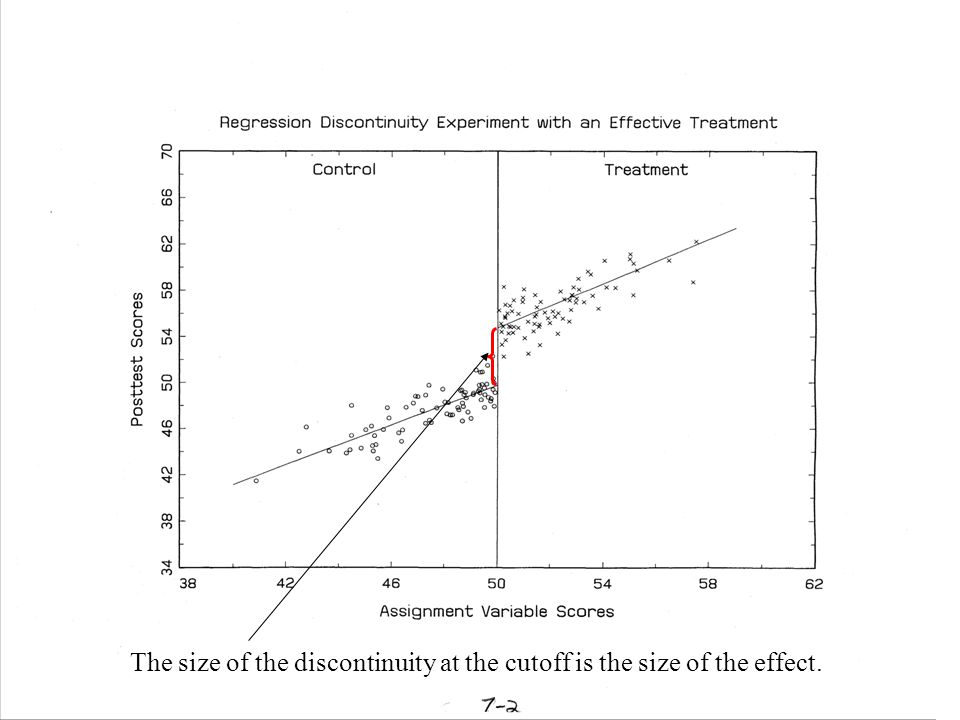
\includegraphics[width=\linewidth]{RD.jpg}
  \end{subfigure} 
\end{figure}
Notice that there are 2 linear regression lines: one before the cutoff and one after cutoff.
These 2 lines have different y-intercepts ($\alpha$) and slope ($\beta$) values.
Say the left line follows the equation:
$$Y_{\text{left}} = \alpha + \beta X_{\text{left}}$$
And the right line follows the equation:
$$Y_{\text{right}} = \gamma + \delta X_{\text{right}}$$
We can try to express these 2 disjointed lines as 1 function by creating an indicator variable that is 1 $\mathbb{I}$, which is 1 if and only if the running variable is above the cutoff:
\begin{gather*}
        \mathbb{I} =
        \begin{cases}
            1 \quad \text{if} \quad X > c \quad \text{(above cutoff)} \\
            0 \quad \text{if} \quad X < c \quad \text{(below cutoff)}
        \end{cases}
\end{gather*}
Then, we can combine the 2 disjointed linear regression lines:
$$\hat{Y} = \alpha + \beta X + (\gamma - \alpha) \times \mathbb{I} + (\delta - \beta) X \times \mathbb{I}$$
Notably, $\gamma - \alpha$ measures the direct jump in the observed variable at the cutoff, and $\delta - \beta$ measures the change in slope.
Lastly, we can horizontally shift the axis to center around $X=c$:
$$\hat{Y} = \alpha + \beta (X-c) + (\gamma - \alpha) \times \mathbb{I} + (\delta - \beta) (X-c) \times \mathbb{I}$$
The treatment effect is determined by $\beta$, the measure of the jump.


\subsection{Assumptions of Regression Discontinuity}
The major assumption here is that all elements near the cut-off are similar.
There are 2 things we have to be aware of because of this.
\\
\textbf{Bandwidth}: Not all units in the treatment and control group are similar to each other; only the ones near the cut-off are. 
The bandwidth is the range around the cut-off in which we consider the units to be similar so that we can compare the 2 groups.
\\
\textbf{Continuity}: This assumption states that amont all units near the cut off, all other covariates should be continuous.
This means that there would not be a jump near the cut-off for any other variable, causing all covariates to be similar among units in the bandwidth and hence preventing any covariates from coming into play. 
\\
\textbf{Bunching}: Bunching is a phenomenon generally in which participants become aware of the cut-off and hence 'bunch' themselves to right above or below the cut-off to be in one group.
An example would be using a specific poverty index to decide government benefits .
If the participants knew about this poverty index and were near the cut-off, they may try to intentionally score themselves to right below the cut-off, in order to receive the benefits.
This would discount our continuity assumption above and hence make direct regression discontinuity analysis obsolete.

\subsection{Sharp and Fuzzy RD}
So far, we have assumed sharp regression discontinuity, which is when one must participate in the treatment if one exceeds the cut-off.
This is not always the case: sometimes exceeding the cut-off will instead allow participants to be eligible in something. 
\\
This then becomes a procedure very similar to noncompliance!
Now, we will think of the cut-off as an instrument variable instead of a treatment variable.
As with noncompliance, we must assume monotonicity (no defiers) and exclusion restrction (the instrument variable does not directly have a causational effect on the outcome).
Similarly, to calculate the local average treatment effect (LATE):
$$\textrm{LATE} = \frac{\textrm{Observed effect of instrument on outcome}}{\textrm{Observed effect of instrument on treatment}} = \frac{E[Y_i|Z_i=1]-E[Y_i|Z_i=0]}{E[T_i|Z_i=1]-E[T_i|Z_i=0]}$$

\end{document}